\section{Reconfiguración de rutas}

\tikzset{potential/.style={every path/.style={dotted}}}

\subsection{Descripción del problema}
Este problema plantea otra provincia de Optilandia, cuyas ciudades están conectadas por rutas pero con ciertos problemas: algunas ciudades no están conectadas y otras poseen varias maneras para viajar entre ellas. Para solucionarlo, el gobierno hará obras en las rutas de modo que haya una y sólo una forma de llegar desde cualquier ciudad a otra, construyendo nuevas rutas o destruyendo rutas existentes. 

Nos piden un algoritmo que, dadas las rutas y los costos de construcción y destrucción, nos diga que rutas hay que destruir y construir para satisfacer el problema de forma que gastemos lo menor posible. Como requisito, la complejidad de este algoritmo no puede ser peor que \textbf{O($n^2log(n)$)}, donde n es la cantidad de ciudades de la provincia.

Veamos un ejemplo del problema. Supongamos que tuvieramos 6 ciudades, con las siguientes rutas iniciales y con los siguientes costos de destrucción expresados en pesos:

\begin{itemize}
	\item Ruta de 1 a 2. Costo de destrucción: 100 pesos.

	\item Ruta de 1 a 4. Costo de destrucción: 230 pesos.

	\item Ruta de 1 a 6. Costo de destrucción: 65 pesos.

	\item Ruta de 2 a 4. Costo de destrucción: 190 pesos.

	\item Ruta de 2 a 6. Costo de destrucción: 300 pesos.

	\item Ruta de 3 a 5. Costo de destrucción: 150 pesos.
\end{itemize}

Por otro lado, tendríamos las siguientes rutas a disposición para construir, con el siguiente costo:

\bigskip

\noindent
\begin{minipage}{0.5\textwidth}
\begin{itemize}
	\item Ruta de 1 a 3. Costo de construcción: 150 pesos.

	\item Ruta de 1 a 5. Costo de construcción: 130 pesos.

	\item Ruta de 2 a 3. Costo de construcción: 190 pesos.

	\item Ruta de 2 a 5. Costo de construcción: 50 pesos.

	\item Ruta de 2 a 6. Costo de construcción: 80 pesos.

	\item Ruta de 3 a 4. Costo de construcción: 300 pesos.

	\item Ruta de 3 a 6. Costo de construcción: 170 pesos.

	\item Ruta de 4 a 5. Costo de construcción: 200 pesos.

	\item Ruta de 4 a 6. Costo de construcción: 150 pesos.

	\item Ruta de 5 a 6. Costo de construcción: 140 pesos.
\end{itemize}
\end{minipage}
\hfill
\begin{minipage}{0.45\textwidth}

	\begin{tikzpicture}[<->, >=latex]
		\begin{scope}[nodeList]
			\node (1) at (0, 2.5) {1};
			\node (2) at (1.5, 5) {2};
			\node (3) at (4.5, 5) {3};
			\node (4) at (6, 2.5) {4};
			\node (5) at (4.5, 0) {5};
			\node (6) at (1.5, 0) {6};
		\end{scope}

		\begin{scope}[pathList]
			\draw (1) -- (2);
			\draw (1) -- (4);
			\draw (1) -- (6);
			\draw (2) -- (4);
			\draw (2) -- (6);
			\draw (3) -- (5);
		\end{scope}

		\begin{scope}[pathList, potential]
			\draw (1) -- (3);
			\draw (1) -- (5);
			\draw (2) -- (3);
			\draw (2) -- (5);
			\draw (3) -- (4);
			\draw (3) -- (6);
			\draw (4) -- (5);
			\draw (4) -- (6);
			\draw (5) -- (6);
		\end{scope}
	\end{tikzpicture}
\end{minipage}

\bigskip

Por lo tanto, la solución más eficiente para dejar un único camino entre todas las ciudades sería:

\begin{enumerate}
	\item Destruir la ruta de 1 a 6, a un costo de 65 pesos

	\item Destruir la ruta de 1 a 2, a un costo de 100 pesos

	\item Construir la ruta de 2 a 5, a un costo de 50 pesos
\end{enumerate}

Lo cual nos daría un costo total de 215 pesos, siendo esta la forma más barata de dejar todas las ciudades conectadas.

\subsection{Desarrollo}
Como es usual, podemos representar a las ciudades como nodos de un grafo y a las rutas como los ejes. Dado que no se especifica si las rutas son de una o dos manos vamos a asumir que las rutas son bidireccionales. Como existen rutas que se pueden destruir y rutas que se pueden crear, vamos a dividir estos ejes en dos conjuntos: el conjunto $C$, que tendrá los ejes con los costos de construcción de rutas; y el conjunto $D$, que va a tener los costos de destrucción. En ambos casos, el costo de destrucción y construcción se representará como el peso del eje correspondiente a esa ruta. Notemos que $C \cup D$ contiene las aristas de un grafo completo. %ejes

Llamaremos $R$ a nuestro grafo solución. El objetivo del algoritmo es que todas las ciudades se conecten solo de una manera, lo que en grafos sería equivalente a que existiese exactamente un camino simple entre todo par de
nodos (es decir, que el grafo solución fuera un árbol). Por lo tanto, \textbf{nuestro objetivo es que $R$ sea el conjunto de aristas de un árbol generador del grafo completo de ejes $C \cup D$.} %ejes

Una vez encontrada la solución, vamos a tener rutas que quedaron intactas y rutas que se construyeron. Al subconjunto de aristas de $C$ que contiene las rutas que deben construirse para lograr la solución óptima lo llamaremos $RC$, y al subconjunto de $D$ que contiene las rutas que hay que mantener lo llamaremos $RD$. Podemos notar que $D - RD$ es el conjunto de rutas que hay que destruir, y que $RD \cup RC$ nos da como resultado la representación de la provincia una vez terminado el plan, osea $RD \cup RC = R$.

El esquema de demostración constará de las siguientes afirmaciones, necesarias para elegir a $RD$ y a $RC$:

\begin{enumerate}
	\item $RD$ tiene que ser un bosque.

	\item $RC$ tiene aristas que conectan a todas las componentes de $RD$, formando su unión un árbol.

	\item $RD$ sera un subgrafo de $D$ tal que para cada componente conexa $D_i \in D$, existe una componente conexa $RD_i$ árbol generador de $D_i$.

	\item Para encontrar al $RD$ óptimo, es necesario que cada $RD_i$ sea árbol generador máximo de $D_i$.
\end{enumerate}

Lo primero que podemos notar es que, si $RD$ no es un bosque, tiene ciclos. Y por ende, si tiene ciclos, no hay manera de que agregando aristas se obtenga un árbol. Pero esto es absurdo, porque vimos que $R$ tiene que ser un árbol. Por ende, $RD$ tiene que ser un bosque. %TODO RD no puede ser un bosque porque son aristas nada mas %grafo

Como $R$ tiene que ser árbol y $RD$ bosque, $RC$ tiene que tener ejes que unan las componentes conexas de $RD$, sin formar ciclos. Además, queremos que el costo de la suma de las aristas que se agreguen sea mínimo. El algoritmo de Kruskal nos va a resolver esto, ya que en la invariante mantiene un bosque y agrega golosamente aristas que conectan componentes hasta alcanzar un árbol. Nos vamos a aprovechar de esto y vamos aplicar Kruskal partiendo del bosque conformado por las aristas de $RD$. Como es bosque, no rompe la invariante y en cada paso conecta a una de las componentes de $RD$ con una arista perteneciente a $C$, agregando dicha arista a $RC$. %grafo

Entonces, sabemos buscar un $RC$ óptimo dado un $RD$. Ahora, tenemos que buscar un $RD$ tal que los costos resultantes sean mínimos. Para esto se nos ocurrió que $RD$ tiene que contener las aristas de un “Bosque Generador Máximo de $D$”, lo cual definimos como un subgrafo de $D$ tal que para cada componente conexa $D_i \in D$, existe una componente conexa $BGM_i \in$ al BGM de $D$ tal que $BGM_i$ es árbol generador máximo de $D_i$.

Veamos por qué el BGM es el bosque óptimo que tenemos para asignar a $RD$. Tenemos a $D$ con componentes conexas $D_1 , D_2 , ... , D_k$, de la cual tomamos $D_i$ con i entre 0 y k. Al sacar un eje cualquiera de $D_i$, si este eje estaba en un ciclo la componente seguirá teniendo los mismos nodos, pero si no, estaríamos dividiendo $D_i$ en dos componentes conexas, llamemoslas $D_{i1}$ y $D_{i2}$, y veamos que esta división de componentes encarece la construcción de $R$ dado este $RD$. 

Llamemos a $RD^{\prime}$ a un bosque subgrafo de $D$ tal que las componentes conexas tienen los mismos nodos que las componentes conexas de $D$ y llamemos $RD^{\prime\prime}$ a otro tal que le quitamos un eje $e$, de la componente conexa $D_i$ dividiéndola en $D_{i1}$ y $D_{i2}$. A lo que queremos llegar es que, si aplicamos Kruskal para conseguir el $RC$ óptimo, con $RD^{\prime\prime}$ el $RC$ resultante tendrá los mismos ejes y uno más, que si le hubiésemos pasado $RD^{\prime}$. Es decir, tendría exactamente los mismos ejes (por ser los de menor costo) más uno que reemplace el eje $e$. Por ende, al costo de agregar los ejes de Kruskal, se le sumaría el de destruir el eje $e$ y agregar un último eje que permita la creación del árbol.Entonces, como exponemos, el costo total de construcción y destrucción sería más caro; por ende, nunca será conveniente quitar ejes que no pertenezcan a ciclos. 

Cuando aplicamos el Kruskal para conseguir el $RC$, estamos uniendo componentes conexas. Como $RD^{\prime\prime}$ tiene una componente más, el $RC$ que parte de $RD^{\prime\prime}$ tendrá $k$ ejes y el que parte de $RD^{\prime}$ tendrá $k-1$, los cuales están todos incluidos en los de $RD^{\prime\prime}$. El algoritmo de Kruskal matiene las componentes conexas y evita que se agreguen ejes que unen nodos dentro de una misma componente para que no se formen ciclos, o sea que si unimos dos componentes tendremos una nueva que contiene a los dos.

Cuando aplicamos el algoritmo, dado $RD^{\prime\prime}$, en algún momento se encontrará con el problema de generar una componente conexa que contenga a $D_{i1}$  y a $D_{i2}$. Para esto, el algoritmo elegirá un eje que nos combine las componentes, al cual llamaremos eje $d$. Al utilizar Kruskal sabemos que, tanto antes como después de agregar el eje $d$, los demás ejes agregados serán los mismos que en el Kruskal de $RD^{\prime}$, puesto que son los mejores posibles en ambos casos. La única diferencia reside en que en $RD^{\prime}$ existe el eje $e$, el que quitamos en $RD^{\prime\prime}$ que une $D_{i1}$ y $D_{i2}$. Esto signfica que en $RD^{\prime}$ tenemos estas dos componentes conectadas sin el costo adicional de borrar $e$ y agregar $d$. Por lo tanto, si llamamos $A$ a la suma de costos de las aristas agregadas por Kruskal que comparten $RD^{\prime}$ y $RD^{\prime\prime}$, y $B$ a la suma de costos de las aristas eliminadas del grafo de entrada que comparten $RD^{\prime}$ y $RD^{\prime\prime}$, tendríamos los siguientes valores:

\begin{center}
	\textbf{costo$(RD^{\prime})$ $=$ $A + B$}

	\textbf{costo$(RD^{\prime\prime})$ $=$ $A + B + e + d$}
	
\end{center}

Y como todos los valores son positivos, porque tanto construir como destruir rutas es costoso (nunca se gana dinero) podemos afirmar que
costo$(RD^{\prime\prime})$ $\geq$ costo$(RD^{\prime})$.

Una deducción que se obtiene de este razonamiento es que sacar mas de un eje empeora todavia más la solución, porque cada vez que le sacamos un eje a un bosque, la cantidad de componentes conexas aumenta en uno. Como dijimos, partir una componente conexa en dos empeora la solución. Podemos usar estas premisas para un razonamiento inductivo que justifica la necesidad de elegir un $RD$ tal que para toda componente conexa $D_i \in D$ exista una componente conexa $RD_i \in RD$ que es árbol generador de $D_i$. En otras palabras, si destruimos el único camino existente entre dos rutas, deberemos necesariamente construir uno nuevo que vuelva a unirlas, y por lo tanto podemos concluir no solo que destruir una ruta útil es perjudicial, sino que destruir una mayor cantidad es más perjudicial aún.

Ahora nos queda ver que el bosque generador máximo es el óptimo. Definimos el costo de $BG$, bosque generador de $D$, como la suma de los pesos de los ejes pertenecientes a $D - BG$ y buscamos que $RD$ sea el bosque generador de costo mínimo. Si $RD$ fuera distinto del BGM de $D$, significaría que su costo es menor que el costo del BGM, lo cual es absurdo porque este es el bosque generador obtenido a partir de la destrucción de las rutas más baratas. Entonces $RD$ tiene que ser el BGM de $D$. Por ende, si usamos Kruskal de manera modificada, nos dará este mismo resultado.

Resumiendo, los pasos a seguir son:

\begin{enumerate}
	\item Obtener los datos de entrada para crear $D$ y $C$

	\item Con $D$ construimos $RD$ (BGM) 

	\item Conseguir el $RC$ óptimo dado $RD$

	\item Calcular los costos de destrucción y construcción
\end{enumerate}

A medida que nos informan las rutas, vamos agregando las rutas en dos listas de ejes, dependiendo si es una existente o si es de construcción. Una vez creadas las listas, corremos Kruskal (en este caso prioriza los ejes caros) de sobre los ejes de destrucción, implementamos Kruskal con Disjoint Set, y para reusar el Disjoint Set en la parte de construcción, este recibe por referencia la estructura. Cuando finaliza el Kruskal recorremos los ejes que nos devuelve y nos fijamos los costos, para después restarle al costo total del grafo $D$ (Ya que eso nos da el costo total de los ejes que destruimos). Después de obtener $RD$, corremos Kruskal de vuelta pero esta vez para buscar el árbol generador mínimo, para esto le tenemos que pasar el Disjoint Set que nos había quedado del anterior Kruskal  y los ejes de las rutas que se pueden construir. Una vez más esto nos devuelve los ejes que vamos a utilizar, calculamos su costo, lo sumamos con el anterior y ya tenemos toda la respuesta.

\subsection{Cota temporal}

Para tener una cota de complejidad temporal sobre nuestro algoritmo, debemos hablar sobre nuestra implementación de Kruskal, ya que es basicamente lo unico que hacemos.
La complejidad de Kruskal está fuertemente atada a la estructura de datos interna utilizada para representar los conjuntos disjuntos. Esta estructura tiene tres funciones en la interfaz, \textit{Init} que inicia el conjunto, \textit{ind} que nos devuelve el representante del conjunto, y \textit{Union} que une los conjuntos. Nosotros lo implementamos con un par de heurísticas \textbf{Union by Rank} y \textbf{Path Compression}, tal que se puede probar que una secuencia de $k$ operaciones de las cuales n son \textit{Init} de estas tres funciones se ejecutan en tiempo $O(k\alpha (n))$ donde $\alpha$ es la inversa de la función de Ackermann. Resumiendo, creamos la estructura, hacemos el sort de la std que tiene una complejidad de $O(nlog(n))$ y en nuestro caso n está acotado por $n^2$ que son la cantidad de aristas máximas que puede haber en un grafo, y por propiedades que exceden el informe(que fueron vistas en clase) nos queda $O(n + m*log(n))$ y como ya vimos que m está acotado $n^2$ podemos también decir que es $O(n^2log(n))$ .Por último, este algoritmo lo corremos dos veces, y para recolectar los costos recorremos las aristas, así que en peor caso es $O(n^2)$, quedando una complejidad temporal del algoritmo de $O(n^2log(n))$ que se ajusta a lo pedido.

\subsection{Experimentacion}

Al experimentar con este problema, nos esperabamos encontrar que el problema solo estuviese definido por la cantidad de ciudades, ya que la cantidad de rutas dependía de la misma (si unimos las rutas existentes con las potenciales, obtenemos un grafo completo). Supusimos que la proporción de rutas existentes y a construir no causaría ninguna diferencia de complejidad, ya que el algoritmo requiere que se recorran todas y la suma siempre da igual para un n dado.

\begin{center}
	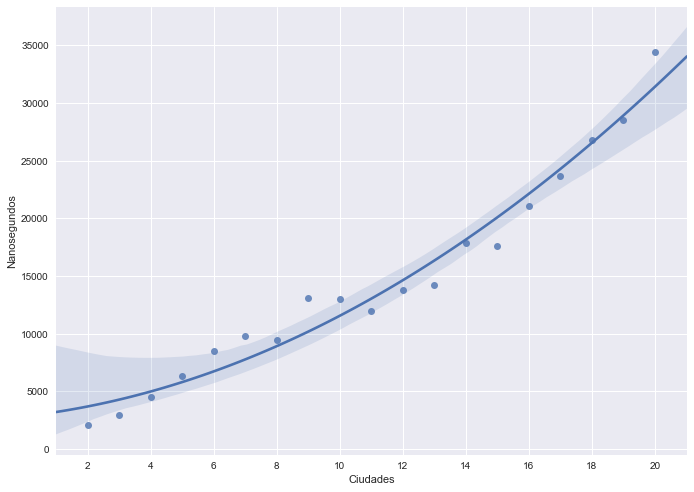
\includegraphics[scale=0.5]{imagenes/ej3-1.png}

	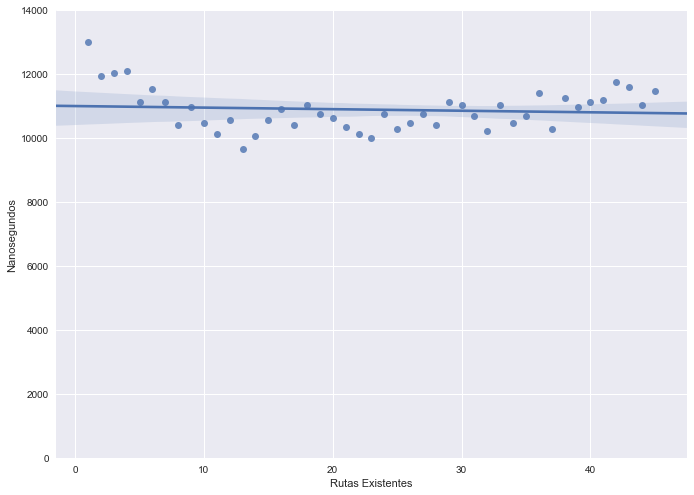
\includegraphics[scale=0.5]{imagenes/ej3-2.png}
\end{center}

Efectivamente, la experimentación confirmó que el algorítmo no se ve afectado por la proporción entre las rutas ya existentes y aquellas a construir. Por otro lado, la cantidad de ciudades tiene un impacto aproximadamente cuadrático. Esto es de esperarse, ya que la complejidad efectiva es $O(n^2log(n))$, pero el aspecto cuadrático es más visible que el logarítmo.
